\chapter{Experiments \& Results}

We detail the experiments from the paper, our implementation, and the results.

\section{Experiments}

The paper included two experiments. The first was to assess the representative power of normalizing flows, where the models were asked to fit 4 different 2D distributions with unnormallized densities $p(x) \propto exp(-U(x))$ which is defiend in the original paper.

\subsection{NICE}

Using the idea of flows, the authors reviewed other work in the field as flows. One of the main comparisons was the coupling layers in the NICE. A coupling layer $f$ is a neural network layer with easy to compute inverse and a trivial Jacobian. For an input vector $\mathbf{z} \in \mathbb{R}^D$, we have
\begin{equation}
f(\mathbf{z}) = (\mathbf{z}_A, g(\mathbf{z}_B,h(\mathbf{z}_A))) 
\end{equation}
\begin{equation}
f^{-1}(\mathbf{z}) = (\mathbf{z}_A, g^{-1}(\mathbf{z}_B,h(\mathbf{z}_A)))
\end{equation}

where $(A,B)$ is a partition of $\{1,2,\dots,D\}$, $h$ is an arbitrary function with input size $|A|$, and $g$ is a coupling law, a function that is invertible for the first argument given the second. In the paper, $h$ is a neural network and $g(a,b)=a+b$, so the Jacobian is just the identity matrix. Since the determinant of the Jacobian is 1, the authors of (variation paper) classify it as a volume-preserving flow.
The authors of the NICE do point out this issue, and introduce a diagonal scaling layer as the last layer of their models. This was not mentioned in the original paper. Moreover, the authors introduced variants NICE-ortho and NICE-perm instead of the original directly, where random orthogonal and permutation matrices are applied to $\mathbf{z}$ before the partition. 

\section{Implementation}

We followed any specifications from the paper as closely as possible, but do note there were parts which are ambiguous. Notably, the term "parameter update" was used for both experiments. While this generally refers to the number of times a parameter in the model is updated, the models for the second part had more than 500000 parameters. Moreover, while the choice of models and optimizers were clear, the actual architecture of the model was not specified well, which made replicating its results non-trivial.

For the first experiment, a ``model" took in a vector from $\mathbb{R}^2$ and returned a multivariate normal distribution independent of the input. The transformations were then applied to this distribution. For NICE, their choice of architecture was unclear, and we have chosen $h$ to be a ReLU network of 4 layers with hidden dimensions of 2. Each model was train for 500000 parameter updates, so they were each trained for different number of iterations. The types of transforms used are radial flow, planar flow, NICE-ortho and NICE-perm. We also introduce NICE-ortho-diag and NICE-perm-diag, which are NICE-ortho and NICE-perm but with diagonal scaling applied as an additional transform.

For the second experiment, we were only able to run and obtain we created encoders and decoders for distributions, allowing one or more transformations in between. The encoder 

For implementing radial flow, we assume that $\beta \geq -\alpha$ and were able to obtain an explicit inverse. We parameterized $\hat{\alpha} = \exp(\alpha)$ to enforce $\alpha > 0$ and $\hat{\beta} = -\alpha + \exp(\beta)$ as per the appendix of the original paper.

\section{Results}

\begin{figure}
\centering
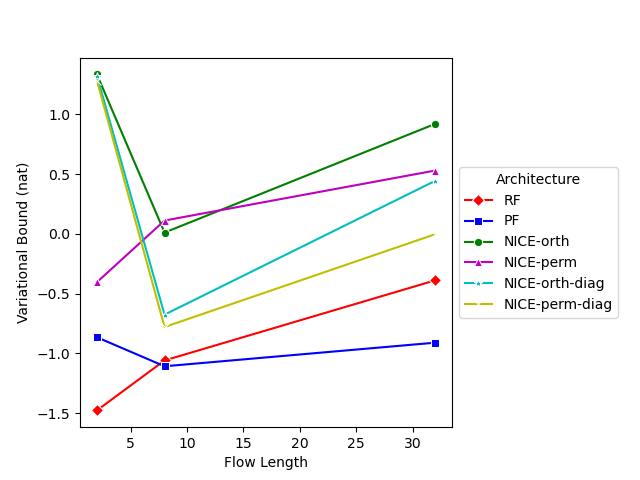
\includegraphics[width=0.45\columnwidth]{u1}
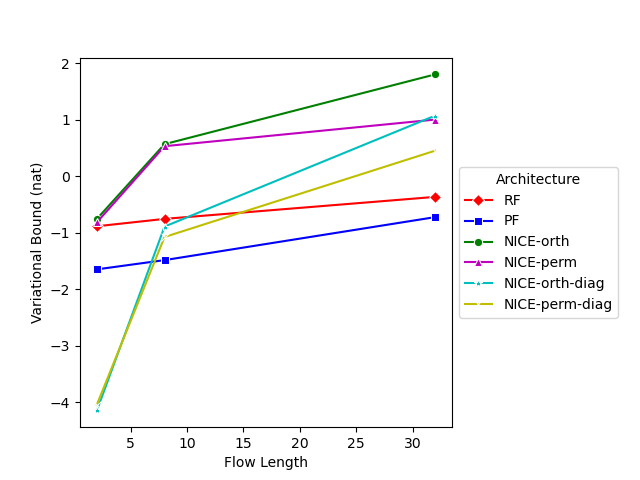
\includegraphics[width=0.45\columnwidth]{u2}
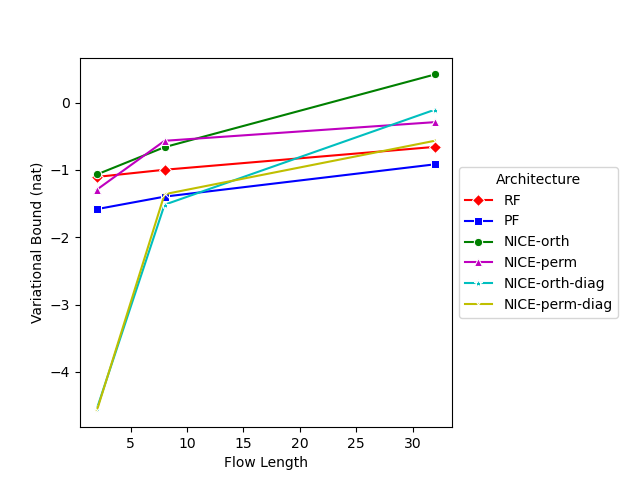
\includegraphics[width=0.45\columnwidth]{u3}
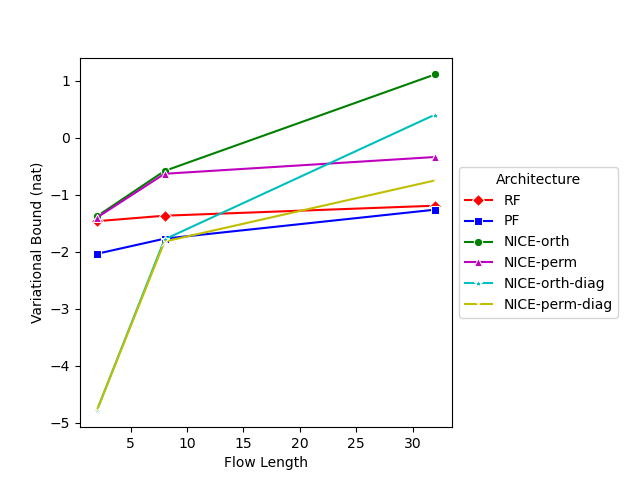
\includegraphics[width=0.45\columnwidth]{u4}
\caption{Variational Bounds of the models with respect to the 4 distributions. Read from top to bottom, left to right.}
\end{figure}

After 50000 parameter updates, the variational bounds are show in Figure 4.1. While the range of values is close to those from the paper, the shapes are visibly inconsistent. We suspect this is due to the ``parameter updates" being iterations or epochs. We do note that among NICE-based models, those with diagonal scaling do perform better than their counterparts.

For the second experiment,